\documentclass{article}
\usepackage[utf8]{inputenc}
\usepackage{amsmath}
\usepackage{graphicx}

\begin{document}

\title{A Spatial Regression Model for Combined Point-Polygon Data}
\author{Sara LaPlante \& Neal Marquez}
\date{December 2018}

\maketitle

\begin{abstract}
A new found focus on reducing inequalities in health outcomes has required that geolocated(point) data be used to understand the geographic risk field of detrimental health outcomes and who lies at the margins for greatest risk. While some data sources provide geographic coordinates of the location that individuals were surveyed, many more data points are representative of larger areal units(polygons). How to harmonize these data sources has been widely contested, but to date, no agreed solution has overcome issues when data is presented in the form of point and polygons. We present a new approach using an approximated integration of a continuous underlying field to incorporate areal units of data of any shape alongside point data for a binomial process.  To test this approach we compare our methodology against previously stated solutions in a simulation environment where the underlying structure of the "risk field" is known. Our analysis finds that the estimated risk field is able to be faithfully recovered in a number of simulation scenarios, out performing previous models. 
\end{abstract}

\section{Introduction}\label{introduction}

The use of continuous spatial models to estimate health risks in very granular well defined locations has seen a boom in the global health field in recent years \cite{Bosco2017, Burke2016, Gething2015, Golding2017, Utazi2018a, Wakefield2017}. The ability to report on estimates of a particular health outcome at any administrative level, shape, and size is an attractive feature for turning research into a policy relevant measure. Estimation of continuous spatial risk fields enable researchers to relay information to policy makers who may have jurisdiction over different administrative areas with differing levels of reach. 

While many have touted the importance of creating more precise metrics for directed health policies\cite{Bhutta2016, Desmond-Hellmann2016}, there is no consensus on the best way to approach creating continuous spatial risk fields, both in terms of methodology and the criteria for data inclusion in a particular analysis. For example, while most of the previous undertakings that have created continuous spatial risk fields for health outcomes have relied on the Demographic and Health Survey (DHS) for inference, whether and how to include other data sources into the analysis is debated. While the DHS provides a reliable data set of over 300 surveys constructed with a multi-stage cluster sampling design in over 90 countries, no one country has been surveyed more than 5 times in the 16 year period between the 2000-2015 period, with many countries only being surveyed on two or less occasions \cite{Burgert-Brucker2016, Gething2015}. This limitation has led several studies to go beyond the inclusion of just DHS data, and incorporate other survey and census enumerations that collect data on the same health events, although data is reported at a different geographic level than required for traditional geospatial analysis \cite{Golding2017, Reiner2018}. The inclusion of data sets from within country surveys, censuses, and registration systems should be seen as particularly urgent as well developed reporting systems become more available. Registration systems offer the best way to analyze health process if the registration system is well defined and comprehensive \cite{AbouZahr2015}.

However, even when we restrict ourselves to the domain of DHS data, the traditional criteria for inclusion for geospatial analysis and estimation of continuous spatial risk fields are data points that have been geolocated to a particular set of coordinates, henceforth referred to as point data. This limits the number of data points for analysis even further as the DHS does not include information of the coordinates associated with particular responses for all survey modules. Again, several studies have attempted to overcome this issue by introducing novel methods of dealing with estimating continuous spatial risk fields from aggregated administrative data, henceforth referred to as polygon data, in the absence of or in conjunction with point data \cite{Golding2017, Reiner2018, Utazi2018a}. 

In this paper, we present a new analytic approach for dealing with polygon data in the estimation of continuous spatial risk fields that more closely resembles the hypothesized data generating process. We begin our discussion with a brief review on the importance of geospatial analysis for the field of public health. We follow up with a review on how other approaches that have attempted to combine point and polygon data for this type of analysis have been flawed in some way and then present a new method for incorporating polygon data into analysis. We then test our model in a simulation framework where the true underlying continuous spatial risk field is known and we sample from the field in a number of different ways, comparing the ability to recreate the underlying field using our new proposed method against a previously proposed method presented in an earlier analysis \cite{Utazi2018a}.

\section{Background}\label{background}

The conclusion of the Millennium Development Goals (MDGs) at the end of 2015 and the subsequent analysis of progress that countries made toward these goals provided as many questions as it answered. The improvements of various health outcomes were evident for many countries, and although not all countries had met the benchmarks set out by the MDGs, most saw serious improvements. These improvements, however, brought up further lines of questioning. Namely, policy makers are now concerned with the how and who of the advancements made during this time period. What changes in health policy, infrastructure, and technologies made this improved state of health possible and who within each of these countries benefited from the changes that were made. 

This shift in focus from country level indicators to how individuals deferentially experience health outcomes has been embodied in the Sustainable Development Goals (SDGs). In response to the demands of policy makers and SDGs we have seen a number of analyses which utilize model based geostatistics to estimate continuous spatial risk fields of negative health outcomes to better understand the inequalities of health outcomes that individuals experience within a country. The DHS has enabled researchers to estimate these fields by providing data that is both representative and well documented, providing the approximate coordinates of where surveys take place up to a known degree of displacement in order to protect the identities of those participating in the survey \cite{Burgert-Brucker2016, Gething2015}. 

A strong limitation of these analysis is that they require all data to be located to a set of coordinates on a spatial field, usually latitude and longitude, in order to be considered for incorporation of data for the estimation of a continuous spatial risk field. This limits us even when only using DHS data, where not all information has been appropriately geotagged. Several studies have previously presented methods for strategies to incorporate polygon data that is representative of larger administrative regions into continuous geospatial analysis.

\subsection{SPDE and Continuous Spatial Risk Fields}

By far, the most used approach to estimating continuous spatial risk fields in health research has been through the use of the the Stochastic Partial Differential Equations (SPDE). The SPDE approach allows one to estimate a continuous Gaussian processes, by way of approximation through a Gaussian Markov Random Field \cite{Lindgren2011}. This approximation allows one to estimate a continuous spatial field in a more traditional statistical model that enables incorporation of covariate fixed effects and uncertainty on the estimated field. For this paper we restrict ourselves to analyzing binomial data, which is a common from of data used in public health to estimate health outcomes. The SPDE model states that we may reconstruct a continuous spatial field by estimating the linear form and parameters seen in equation \ref{binomSPDE}.

\begin{align}\label{binomSPDE}\begin{split}
    i,j \in \{1, \dots, n\}\\
    Y_i \sim \text{Binomial}(N_i, \hat{p}_i) \\
    \text{logit}(\hat{p}_i) = X_i \hat{\boldsymbol{\beta}} + \eta(s_i)  \\
    \boldsymbol{\eta} \sim \text{MVN}(\boldsymbol{0}, \boldsymbol{\Sigma}) \\
    \Sigma_{ij} = \frac{\hat{\sigma}^2_\eta}{2^{\nu-1} \Gamma(\nu)}
        (\hat{\kappa} ||s_i - s_j||)^\nu K_\nu(\hat{\kappa} ||s_i - s_j||) \\
    \Sigma_{ij} = \text{Cov}(\eta(s_i) , \eta(s_j))
\end{split}\end{align}

For any given observation $i$ that takes place at point $s_i$ on a continuous spatial field of interest we may estimate the parameters seen with a hat designation in equation \ref{binomSPDE} where $p_i$ is the probability of some health related event. More often than not, a Bayesian hierarchical approach is used with hyper-priors for the parameters $\kappa$ and $\sigma$ \cite{Burke2016, Reiner2018, Utazi2018a, Wakefield2017} and an Integrated Nested Laplace Approximation (INLA) to the posterior \cite{Rue2009}, however, other studies from fields outside of public health have utilized Restricted Maximum Likelihood (REML) to fit the parameters \cite{Gruss2018} using the software Template Model Builder (TMB) \cite{Kristensen2016a}.

\subsection{Previous Approaches to Polygon Data Utilization}

While many studies simply have chosen to exclude polygon data from their analysis \cite{Burke2016, Wakefield2017} several authors have taken on approaches for dealing with polygon data in continuous spatial field analysis. In studies related to the Global Burden of Disease analysis, the common approach has been to incorporate data by way of re-sampling such that point data is derived from polygon data by a population weighted placement of J representative points which are constructed by way of K-means clustering \cite{Golding2017, Reiner2018}. In this way the model deals only with pseudo constructed points from polygons and may be incorporated into the analysis in a typical fashion. Others have previously commented on the problematic nature of this approach \cite{Wakefield2017} including the authors themselves calling for a more robust approach for dealing with the inclusion of polygon data that more appropriately deals with point uncertainty which is artificially minimized through point re-sampling \cite{Golding2017}.

More recently, models that take a more sophisticated approach have been introduced to the family of geospatial models that utilizes the SPDE approximation. Building off of the work of Moraga et al \cite{Moraga2017} Utazi et al in 2018 described a method for spatial dis-aggregation of areal units to continuous spatial risk field. In their paper they describe a methodology for estimating continuous fields from only non-overlapping polygon data and provide a simulation framework for testing their model, although they do not compare their model to other proposed approaches such as the re-sampling method. The crux of their argument is that polygon data can be used in an estimation process that estimates two separate and separable latent processes as shown in equation \ref{utaziModel}.

\begin{align}\label{utaziModel}\begin{split}
    i \in \{1, \dots, n_{\mathcal{A}}, n_{\mathcal{A}} + 1, \dots, n_{\mathcal{A}} + n_p\}\\
    Y_i \sim \text{Binomial}(N_i, \hat{p}_i) \\
    \text{logit}(p_i) = \overset{\sim}{x}_i \boldsymbol{\beta} + |\mathcal{A}_i|^{-1} \int_{\mathcal{A}_i} \eta(\boldsymbol{s}) d\boldsymbol{s} + \phi_i \\
    \text{logit}(p_i) = x_i \boldsymbol{\beta} + \eta(\boldsymbol{s}_i) + \phi_{\mathcal{A}_i}
\end{split}\end{align}

An in depth description of the model is provided in the original paper of this model, however, several conceptual limitations of this approach were not addressed. Perhaps the strongest limitation from this approach is the way that covariates are handled in the model. Utazi et al state that for polygon data the covariate value associated with an observation is simply the integral or block average of a given spatial covariate. This approach is problematic for two reasons. If we believe that for data reported from a polygon is representative then we would expect that the stochastic process that produces observations is an average or integral of the population weighted area of the probabilities themselves not the integral of the covariates (and the spatial latent field). This is especially problematic because it violates known issues of ecological fallacy, where the correlation of covariates is differential to a particular outcome depending on the level of geographic specificity used in the analysis \cite{Dark2007, Openshaw1984}. Secondly, if we expect that the continuous latent spatial field operates independent of arbitrary administrative borders it is unclear how the inclusion of a latent CAR component, $\phi$, contributes to this estimation. One could envision how a policy implemented in a particular region could have an effect on a particular health outcome, however, as currently presented, the model restricts analysis to polygons that are non-overlapping and comprehensive of the entire study area of concern, a criteria that is not difficult to find contradictions to, even within DHS data. 

In order to address issues of proper uncertainty of polygon data, correctly handling covariate effects, and enabling the ability to use polygon data even in the case of overlapping areas we present a new model outlined in the next section.

\section{Methods}\label{methods}

If we believe that the true data generating process comes from a structure that is shown in equation \ref{binomSPDE} then we may work from here on approximating the likelihood of polygon samples. Let us consider that for a given polygon the average probability for a given area may be approximated by taking the population weighted integral of the continuous spatial risk filed of a given area. 

\begin{align}\label{pIntegral}
p_{\mathcal{A}_i} = |\mathcal{A}_i|^{-1}\int_{\mathcal{A}_i} \boldsymbol{p}_i * \text{popWeight}_i ~ d\boldsymbol{p}
\end{align}

Because the values of $\boldsymbol{p}$ on the right hand side of this equation are difficult to integrate we may approximate this integration numerically via Riemann sum approximation. The incorporation of population weights is trivial in this approximation and simplifies to equation 4.

\begin{align}\label{pRiemann}
p_{\mathcal{A}_i} = \sum_{j \in \mathcal{A}_i} p_i * \text{popWeight}_i
\end{align}

This approximation enables us to get the first moment of our expected likelihood for a polygon sample. We may then use a binomial likelihood and the estimated $p_{\mathcal{A}_i}$ to evaluate the data. The model is not inhibited by the differential level of covariate effects as the covariate correlation level is estimated at the point level even when polygon data is presented. In addition, The incorporation of any polygon may be added to this process and does not require that polygons comprehensively cover the area or that they must not overlap as in the Utazi model. Additionally this model more appropriately handles uncertainty as the estimation of points are known to be correlated in space and observing a polygon rather than a point lowers uncertainty for a given area although not to the same extent that observing point data would across the area.

It should be noted that this approximation ignores the fact that these observations came from a convolution of binomials rather than a true binomial process. The consequence of this is that there is an assumption of greater than expected variance, the second moment, for polygon data. While we do not expect this to effect our analysis to a great extent, known approximations to the convolutions of binomials are available and will be tested in the near future \cite{Liu2017}.

\section{Model Testing}\label{model testing}

To test the performance of our model, we simulate a wide variety of randomly-generated risk fields to mimic potential geographies found in practical applications. We then sample from these fields to mimic sampling that would occur in real scientific research and subsequently run our proposed model on the sample to see if it can recover the true generated field. Since we know the true parameters fed into each simulation, we will be able to measure how closely our model was able to estimate the true risk field it is given.

As a point of reference, we have chosen to test a previously proposed model alongside our own. This will enable us to see where our model does (or does not) provide improvements. The model we have chosen for comparison is that proposed by Utazi, et al. (2018). For ease of use, we will refer to this as the ``Utazi model'' and to our model as the ``Riemann model''. (This name comes from the fact that our model uses Riemann sums to approximate the model's main integral.)

To generate the 450 risk fields we will use in our simulations, we begin with a 60x60 pixel grid. We assume that the risk for each pixel in the grid is generated by an inverse logit of an intercept, one covariate, and a latent spatial field:

\begin{align}\label{lin}
p_i=\text{inverse logit}(\beta_0+\beta_1x+ \eta(s_i)).
\end{align}

To create diversity in the fields, we vary the following: covariate type, covariate value, and spatial range. The intercept we hold constant ($\beta_0=-2$ for all fields). Since in practice, a variety of covariates generate risk fields, we consider three types: a truly random covariate, a covariate correlated across space, and a covariate constant across large geographic regions. Figure \ref{fig:simPlot} shows these scenarios.

\begin{figure}[ht]
    \centering
    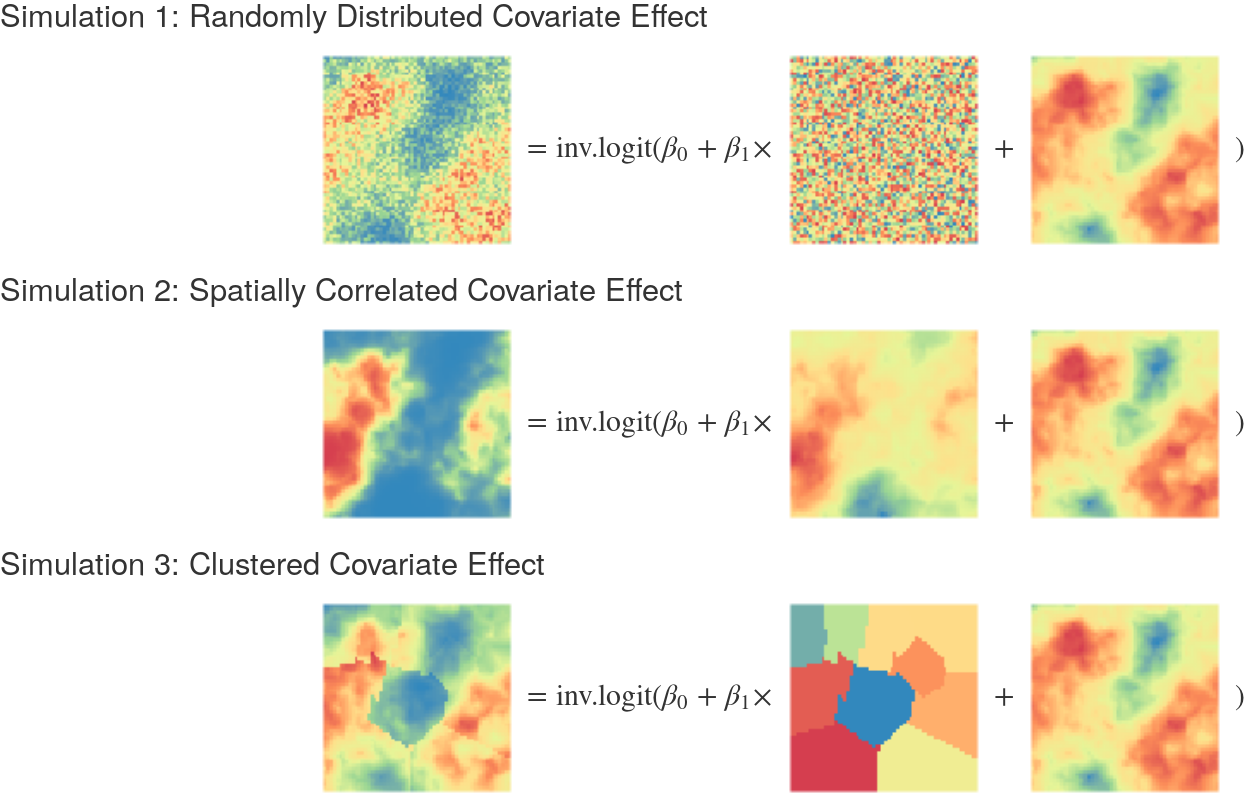
\includegraphics[width=.7\textwidth]{./figures/covariateeffects.png}
    \caption{Examples of three simulated risk fields using each of the three covariate types and the same latent spatial field. The risk field on the left is found by plugging the components shown on the right into the inverse logit function, pixel by pixel, from a transformation of a linear combination of the $\boldsymbol{\beta}$ parameters, a single covariate, and a latent spatial process.}
    \label{fig:simPlot}
\end{figure} 

For each of these covariate types, we generate fields with covariate values in $\{-2, -.5, .2, .4, 2\}$. We also vary the spatial range in $\{.3, .5, .7\}$. This measures the spatial correlation of the spatial components in our model (either the latent spatial field alone or both the latent spatial field and the spatially-correlated  covariate). Finally, we use 10 random seeds for each combination of values to ensure randomness in our true fields. The components that go into these 450 risk fields are shown in Figure \ref{fig:parPlot}.

 \begin{figure}[ht]
    \centering
    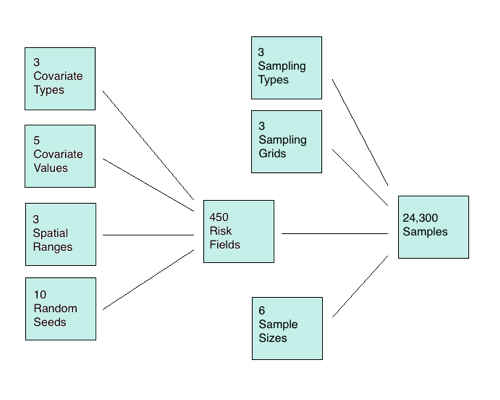
\includegraphics[width=.7\textwidth]{./figures/samplingexplained.png}
    \caption{A visual aid to understanding how we generate each of the 450 risk fields and 24,300 samples in our simulation.}
    \label{fig:parPlot}
\end{figure}

We sample from each of these generated risk fields to create 24,300 samples for model testing. Each sample is a combination of a risk field, one of three sampling types, one of three sampling grids, and one of six sample sizes. By sampling types, we mean whether we simulate that the data came to us as polygons only, a combination of non-overlapping points and polygons, or a combination of overlapping points and polygons. In an ideal world, we would only receive point data with a large sample size, but the literature has already addressed this scenario well and our model will perform identically to many well-tested models. We focus on the remaining models which include either a mixture of point and polygon data or exclusively polygon data. Figure \ref{fig:samplingPlot} shows what these types of samples would look like given the true risk field shown.

\begin{figure}[ht]
    \centering
    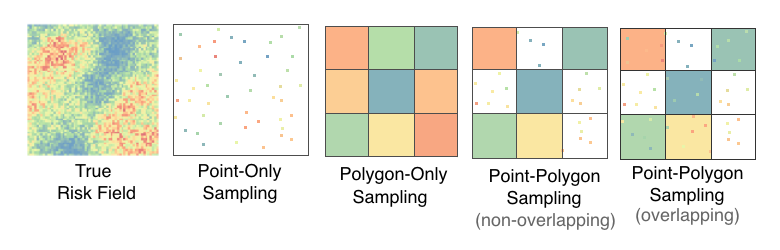
\includegraphics[width=.7\textwidth]{./figures/samplingtypes2.png}
    \caption{An example of a simulated true risk field (left) and the four sampling types (right). We exclude point-only sampling in our simulation.}
    \label{fig:samplingPlot}
\end{figure}

The sampling grids allow us to vary the size of the polygons we sample (3x3, 5x5, 9x9). We choose sample sizes uniformly from 50 to 300.

After creating this simulation environment, we test both the Utazi and Riemann models on each of the 24,300 samples. The Riemann model fits using restricted maximum likelihood via R's Template Model Builder. The Utazi model fits using a combination of Bayesian inferene and integrated nested Laplace approximation via R's INLA package as outlined in Utazi, et al. (2018). Both models estimate a $\beta_0$ value, a  $\beta_1$ value, and the latent spatial field. We plug these values into the assumed form of the pixel probability to predict a risk value for each pixel in the 60x60 grid. 

The Riemann model produces a Hessian matrix for estimated parameters which we use to estimate the standard errors for our continuous spatial risk field. The hessian allows us to produce uncertainty estimates for each of our 3600 pixels by simulation from the hessian using a multivariate normal distribution and an inverse logit transformation of the linear combination as seen in Equation \ref{lin}. In contrast the Utazi model returns the posterior of each pixel as it uses a Bayesian estimation process with priors and hyper-priors as described previously \cite{Utazi2018a}.

\section{Results}\label{results}

\begin{itemize}
\item  Discuss model performance across different stratification's and performance checks
\item RMSE and Coverage at the pixel level and Beta bias
\end{itemize}

\section{Discussion}\label{discussion}

In this paper we present a new method for incorporating polygon data into spatial risk field estimation with binomial data. Though previous methods have been presented to deal with this problem, they have not been compared in a simulation environment against other models. In our analysis we show that in comparison to a previously proposed model, the newly presented Riemann model on average provides marginal improvements in latent field RMSE and accurate coverage of the latent field in the 95\% confidence intervals. Though not reported here we also tested our model in a similar simulation framework against the re-sampling strategy employed by several previous authors \cite{Golding2017, Reiner2018}, however, this model produced considerably worse estimates for all predictive validity metrics in comparison to the Utazi and Riemann methods and for this reason was not discussed in the simulation framework.  

As shown previously, when the analysis of the simulated results excluded the most coarse form of polygon only data sampling (3x3 grid) with no point data, the marginal benefits provided by the Utazi model for Beta bias were not of great consequence and overlapped with no improvement in the 95\% confidence interval. We should hesitate to ever use any model that attempts to estimate a continuous spatial field from a few very course polygons and no point data as the ability to evaluate such a model becomes very difficult. For example, both the Utazi and the Riemann models standard errors of the beta coefficients reached upwards of 20 in the 3x3 polygon only sampling frame. This large uncertainty compared to any of the true values of the beta coefficients used in the simulation process should give us pause on the use of a geospatial model in this context. Furthermore, the reporting of estimates from any of these models should be reported at aggregated areas that are testable to the given data that was used to create them, even if we model the data as continuous and estimate it with a continuous spatial field. Though we present a model here that outperforms previous models in the polygon only sampling scenario for estimating continuous spatial risk fields, when the polygons are sufficiently granular, we urge that researchers use extreme caution in this estimation process as the ability to truly test the continuous field in the absence of point data is not a well defined process. 

An additional limitation of our model is that the use of the binomial likelihood as a way to estimate polygon data that comes from different locations within the polygon with different probabilities ignores the convolution of binomials process \cite{Butler1993}. Future analysis should better deal with this problem by way of known approximations such as the Pearson or Saddle point approximation \cite{Liu2017}.

To show the extent to which our model produces estimates that differ from previous estimates, future work will seek to include an application to real word health data from both the DHS as well as the Multiple Indicator Cluster Survey (MICS), a project that strongly mimics the process of the DHS. In particular an application to estimating the risk of under 5 mortality within the Dominican Republic offers a robust testing opportunity for our model. The Dominican Republic had a number of both point and polygon samples collected from both MICS and DHS between the years 2000 and 2015. In addition, child mortality is seen as an important overall health indicator as it is a strong correlate of both maternal and reproductive health as well as known indicator for access to health facilities \cite{AbouZahr2015}.

Many other analyses discussed in this paper incorporate not only a spatial dimension, but also, a temporal dimension. The importance of not only estimating differences within a geography but also changes overtime, is essential for evaluating the health performance of a particular country. Our presented model can trivially incorporate temporal dimension to it in addition to being able to incorporate polygons, from which temporal observations need not be observed at every time period.

The importance of building estimates of continuous spatial risk fields is of great importance to the field of public health. When generating estimates for these fields it is essential that we do so in way that minimizes error of the true field while providing accurate estimates of uncertainty. Our presented model provides the best estimation process when compared to previous models and should be considered for use in geospatial health outcome estimation.

\newpage

\bibliographystyle{plain}
\bibliography{ppp.bib}

\end{document}
